% Reminder: Verify that the first three assigned questions (14.1 #9, #11, #15) match the PDF and the other required book.
\documentclass[11pt]{article}
\usepackage[margin=0.85in]{geometry}
\usepackage{amsmath,amssymb,mathtools,enumitem,booktabs}
\usepackage[T1]{fontenc}
\usepackage{lmodern}
\usepackage{pgfplots}
\pgfplotsset{compat=1.18}
\usepackage{needspace}
\usepackage[colorlinks=true,linkcolor=blue]{hyperref}
\setlength{\parindent}{0pt}
\setlength{\parskip}{0.4em}
\setlength{\emergencystretch}{2em}
\newcommand{\ex}[1]{\Needspace{8\baselineskip}\subsection*{Exercise #1}}
\newcommand{\ans}[1]{\boxed{#1}}
\newcommand{\vv}[1]{\left\langle #1\right\rangle}
\newcommand{\ii}{\mathbf i}\newcommand{\jj}{\mathbf j}\newcommand{\kk}{\mathbf k}
\newcommand{\cp}[6]{\begin{vmatrix}\ii&\jj&\kk\\#1&#2&#3\\#4&#5&#6\end{vmatrix}}
\pgfplotsset{every axis/.append style={width=.70\linewidth,height=6cm,xlabel={$x$},ylabel={$y$},zlabel={$z$},view={125}{25},grid=major}}
\newcommand{\surf}[4]{\begin{center}\begin{tikzpicture}\begin{axis}[#1]\addplot3[surf,shader=interp,samples=19,samples y=19,opacity=.78] ({#2},{#3},{#4});\end{axis}\end{tikzpicture}\end{center}}
\newcommand{\curve}[4]{\begin{center}\begin{tikzpicture}\begin{axis}[#1]\addplot3[blue,thick,samples=180,samples y=0,variable=t] ({#2},{#3},{#4});\end{axis}\end{tikzpicture}\end{center}}
\title{Chapter 14: Partial Derivatives\\Worked solutions to the assigned exercises}
\author{Anish Kumar}\date{}\begin{document}\maketitle
\noindent\fbox{\parbox{0.94\linewidth}{\textbf{Reminder to myself:} I need to verify that the first three assigned questions (14.1 \#9, \#11, and \#15) match between this PDF and the other book I am supposed to use. This comparison is still pending.}}
\medskip

\noindent\textbf{Source and scope.} Stewart, Clegg, and Watson, \emph{Calculus}, ninth edition, multivariable volume. Only Chapter 14 exercises in \texttt{assignment\_manifest.json} are included. Each entry gives a short description followed by the method, intermediate steps, and conclusion. At your request, four inaccessible assigned entries are skipped: 14.3 \#104 (this section ends at \#101) and 14.8 \#17, \#19, \#21 (they refer to Section 4.7 \#3, \#7, \#25 outside this volume). This file contains the other 103 assigned exercises; add the skipped items after receiving the updated assignment.
\medskip

\noindent\textbf{Reading the notation.} A subscript such as $f_x$ means a partial derivative; hold the other variables fixed. A boxed expression marks a result. A decimal approximation is indicated by $\approx$; exact fractions and radicals are kept when possible.
\medskip

\noindent\textbf{Textbook navigation (printed pages / PDF pages).}
\begin{center}\begin{tabular}{lll}\toprule Section & Printed exercise pages & PDF pages\\\midrule
14.1 & 946--950 & 309--313\\
14.2 & 960 & 323\\
14.3 & 970--973 & 333--336\\
14.4 & 981--982 & 344--345\\
14.5 & 991--992 & 354--355\\
14.6 & 1005--1007 & 368--370\\
14.7 & 1017--1018 & 380--381\\
14.8 & 1026--1027 & 389--390\\\bottomrule\end{tabular}\end{center}
\clearpage\tableofcontents
\clearpage\section*{14.1 Functions of Several Variables}\addcontentsline{toc}{section}{14.1 Functions of Several Variables}
\Needspace{25\baselineskip}
\ex{9}
\textbf{Question.} Find and sketch the domain of $g(x,y)=\sqrt{x}+\sqrt{4-4x^2-y^2}$.

\textbf{Worked solution.}
For $g(x,y)=\sqrt{x}+\sqrt{4-4x^2-y^2}$, both radicands must be nonnegative:
\[x\ge0,\qquad4x^2+y^2\le4.\]
Thus the domain is the closed right half of the ellipse $x^2+y^2/4\le1$. The boundary and the interior are included because neither root is a denominator.
\begin{center}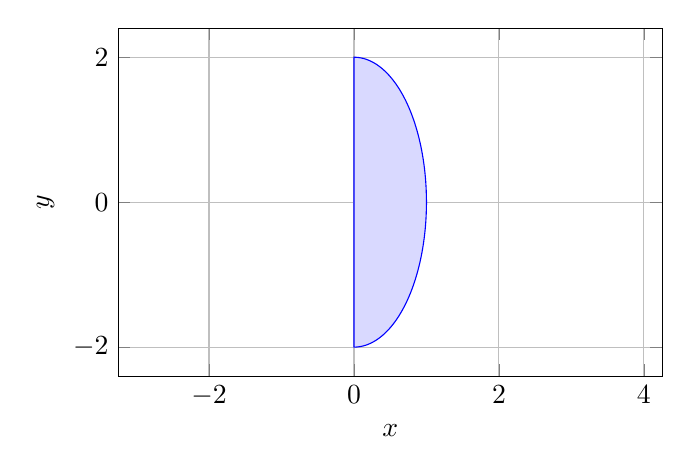
\begin{tikzpicture}\begin{axis}[view={0}{90},axis equal,xmin=-.3,xmax=1.3,ymin=-2.4,ymax=2.4]\addplot[blue,fill=blue!15,domain=-90:90,samples=100] ({cos(x)},{2*sin(x)})\closedcycle;\end{axis}\end{tikzpicture}\end{center}
\Needspace{25\baselineskip}
\ex{11}
\textbf{Question.} Find and sketch the domain of $g(x,y)=(x-y)/(x+y)$.

\textbf{Worked solution.}
The quotient $(x-y)/(x+y)$ exists exactly when $x+y\ne0$. Hence $\ans{D=\{(x,y):y\ne-x\}}$: the entire plane with one line removed. The dashed line in the sketch is excluded; both sides are allowed.
\begin{center}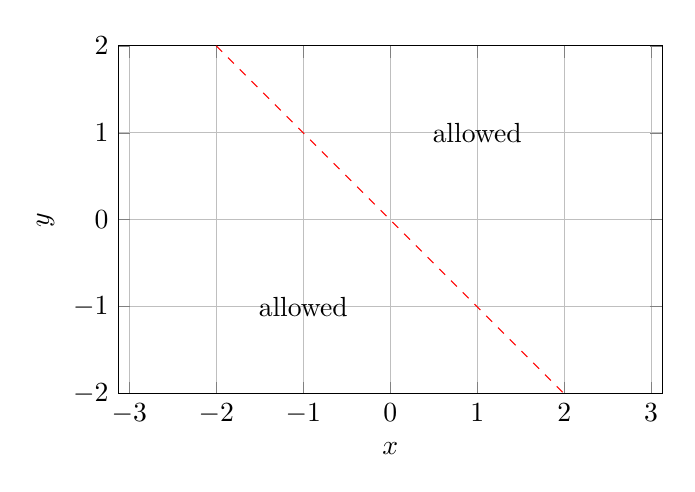
\begin{tikzpicture}\begin{axis}[view={0}{90},xmin=-2,xmax=2,ymin=-2,ymax=2,axis equal]\addplot[red,dashed,domain=-2:2]{-x};\node at (axis cs:1,1){allowed};\node at (axis cs:-1,-1){allowed};\end{axis}\end{tikzpicture}\end{center}
\Needspace{25\baselineskip}
\ex{15}
\textbf{Question.} Find and sketch the domain of $f(x,y,z)=\sqrt{4-x^2}+\sqrt{9-y^2}+\sqrt{1-z^2}$.

\textbf{Worked solution.}
Each coordinate has its own root restriction:
\[4-x^2\ge0\Rightarrow-2\le x\le2,\quad9-y^2\ge0\Rightarrow-3\le y\le3,\quad1-z^2\ge0\Rightarrow-1\le z\le1.\]
Therefore $\ans{D=[-2,2]\times[-3,3]\times[-1,1]}$, a solid rectangular box, including all faces, edges, and vertices.
\begin{center}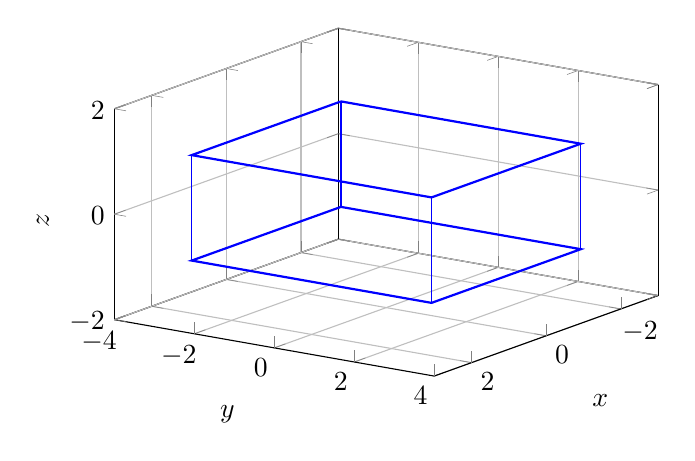
\begin{tikzpicture}\begin{axis}[xmin=-3,xmax=3,ymin=-4,ymax=4,zmin=-2,zmax=2]\addplot3[blue,thick] coordinates {(-2,-3,-1)(2,-3,-1)(2,3,-1)(-2,3,-1)(-2,-3,-1)};\addplot3[blue,thick] coordinates {(-2,-3,1)(2,-3,1)(2,3,1)(-2,3,1)(-2,-3,1)};\addplot3[blue] coordinates {(-2,-3,-1)(-2,-3,1)};\addplot3[blue] coordinates {(2,-3,-1)(2,-3,1)};\addplot3[blue] coordinates {(2,3,-1)(2,3,1)};\addplot3[blue] coordinates {(-2,3,-1)(-2,3,1)};\end{axis}\end{tikzpicture}\end{center}
\ex{19}
\textbf{Question.} Use the wind-chill table for $W=f(T,v)$ to evaluate $f(-15,40)$, solve $f(-20,v)=-30$ and $f(T,20)=-49$, and interpret the slices $f(-5,v)$ and $f(T,50)$. Here $T$ is in degrees Celsius and $v$ in km/h.

\textbf{Worked solution.}
\begin{enumerate}[label=(\alph*)]
\item Table 1 gives $\ans{f(-15,40)=-27}$. At an actual temperature of $-15^\circ$C with wind $40$ km/h, the perceived temperature is $-27^\circ$C.
\item $f(-20,v)=-30$ asks which wind speed makes $-20^\circ$C feel like $-30^\circ$C. In the $T=-20$ row, $-30$ occurs at $\ans{v=20\text{ km/h}}$.
\item $f(T,20)=-49$ asks for actual temperature when wind is $20$ km/h and perceived temperature is $-49^\circ$C. In that column, $\ans{T=-35^\circ\mathrm C}$.
\item $W=f(-5,v)$ holds actual temperature fixed at $-5^\circ$C and varies wind speed. The values are nonincreasing as $v$ rises: stronger wind lowers perceived temperature.
\item $W=f(T,50)$ holds wind speed fixed at $50$ km/h and varies actual temperature. The values rise with $T$: warmer air raises perceived temperature.
\end{enumerate}
\Needspace{25\baselineskip}
\ex{25}
\textbf{Question.} Sketch the surface $z=10-4x-5y$.

\textbf{Worked solution.}
$z=10-4x-5y$ is a plane. Setting the other two coordinates to zero gives intercepts $(5/2,0,0)$, $(0,2,0)$, and $(0,0,10)$. These three noncollinear points determine the plane; increasing $x$ or $y$ lowers $z$.
\surf{domain=-1:3,y domain=-1:3}{x}{y}{10-4*x-5*y}
\Needspace{25\baselineskip}
\ex{29}
\textbf{Question.} Sketch the surface $z=x^2+4y^2+1$.

\textbf{Worked solution.}
$z=x^2+4y^2+1$ is an elliptic paraboloid opening upward. Its smallest value is $1$, at the vertex $(0,0,1)$. In $y=0$ the trace is $z=x^2+1$; in $x=0$ it is $z=4y^2+1$. A horizontal trace $z=k>1$ satisfies $x^2+4y^2=k-1$ and is an ellipse.
\surf{domain=-2:2,y domain=-1:1}{x}{y}{x^2+4*y^2+1}
\Needspace{25\baselineskip}
\ex{45}
\textbf{Question.} Draw several level curves of $f(x,y)=x^2-y^2$.

\textbf{Worked solution.}
Set $f=k$: $\ans{x^2-y^2=k}$. For $k>0$ these hyperbolas open along $x$ with vertices $(\pm\sqrt{k},0)$; for $k<0$ they open along $y$ with vertices $(0,\pm\sqrt{-k})$. At $k=0$ the contour is the two lines $y=\pm x$. All nonzero contours have these same asymptotes. Blue curves show $k=1,4$; red curves show $k=-1,-4$; dashed lines show $k=0$.
\begin{center}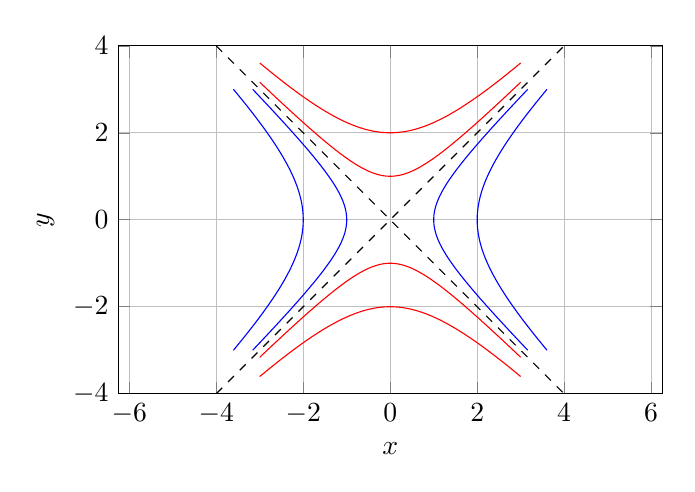
\begin{tikzpicture}\begin{axis}[view={0}{90},axis equal,xmin=-4,xmax=4,ymin=-4,ymax=4]\foreach \c in {1,4}{\addplot[blue,domain=-3:3,samples=90] ({sqrt(x^2+\c)},x);\addplot[blue,domain=-3:3,samples=90] ({-sqrt(x^2+\c)},x);\addplot[red,domain=-3:3,samples=90] {sqrt(x^2+\c)};\addplot[red,domain=-3:3,samples=90] {-sqrt(x^2+\c)};}\addplot[black,dashed,domain=-4:4]{x};\addplot[black,dashed,domain=-4:4]{-x};\end{axis}\end{tikzpicture}\end{center}
\Needspace{25\baselineskip}
\ex{47}
\textbf{Question.} Draw several level curves of $f(x,y)=\sqrt{x}+y$.

\textbf{Worked solution.}
$\sqrt{x}+y=k$ rearranges to $\ans{y=k-\sqrt{x},\ x\ge0}$. Each level is a vertical translate of the same decreasing square-root curve and begins at $(0,k)$. The sketch uses $k=-2,-1,0,1,2$, ordered from bottom to top.
\begin{center}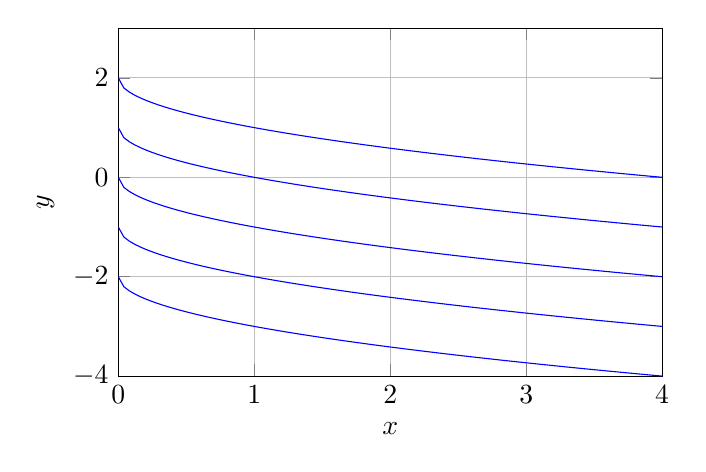
\begin{tikzpicture}\begin{axis}[view={0}{90},xmin=0,xmax=4,ymin=-4,ymax=3]\foreach \c in {-2,-1,0,1,2}{\addplot[blue,domain=0:4,samples=100]{\c-sqrt(x)};}\end{axis}\end{tikzpicture}\end{center}
\Needspace{25\baselineskip}
\ex{49}
\textbf{Question.} Draw several level curves of $f(x,y)=ye^x$.

\textbf{Worked solution.}
$ye^x=k$ gives $\ans{y=ke^{-x}}$. Since $e^{-x}>0$, positive levels lie above the $x$ axis, negative levels below it, and the zero level is $y=0$. All approach the $x$ axis as $x\to\infty$. The sketch uses $k=-2,-1,0,1,2$, ordered from bottom to top.
\begin{center}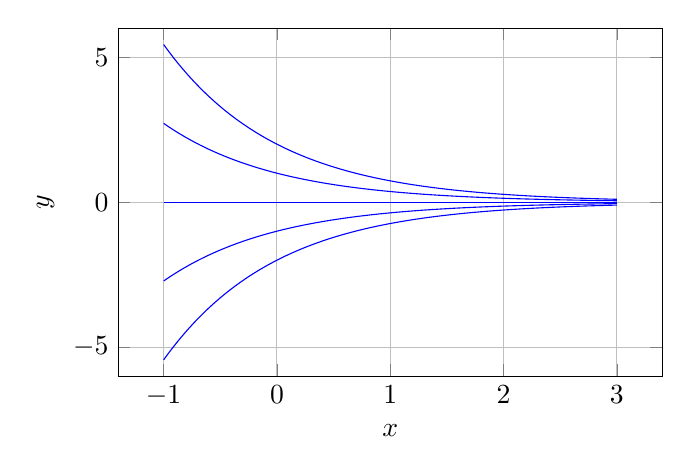
\begin{tikzpicture}\begin{axis}[view={0}{90},domain=-1:3,ymin=-6,ymax=6]\foreach \c in {-2,-1,0,1,2}{\addplot[blue,samples=90]{\c*exp(-x)};}\end{axis}\end{tikzpicture}\end{center}
\Needspace{25\baselineskip}
\ex{51}
\textbf{Question.} Draw several level curves of $f(x,y)=\sqrt[3]{x^2+y^2}$.

\textbf{Worked solution.}
Cubing $\sqrt[3]{x^2+y^2}=k$ gives $x^2+y^2=k^3$. The left side is nonnegative, so $k\ge0$. For $k>0$ the level is a circle centered at the origin with radius $\ans{k^{3/2}}$. At $k=0$ it is the origin; negative levels are empty. The plotted circles correspond to $k=1,1.5,2$, from smallest to largest.
\begin{center}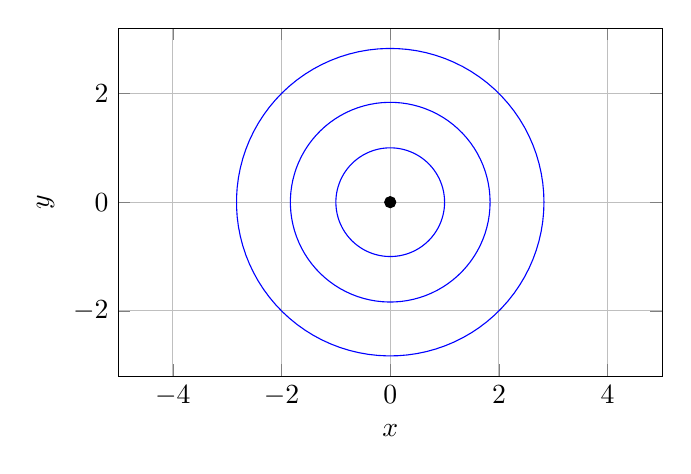
\begin{tikzpicture}\begin{axis}[view={0}{90},axis equal,xmin=-3.2,xmax=3.2,ymin=-3.2,ymax=3.2]\foreach \r in {1,1.8371,2.8284}{\addplot[blue,domain=0:360,samples=100] ({\r*cos(x)},{\r*sin(x)});}\addplot[only marks] coordinates {(0,0)};\end{axis}\end{tikzpicture}\end{center}
\ex{61}
\textbf{Question.} Match $z=\sin(xy)$ to a surface A--F and a contour map I--VI in the textbook, explaining both choices.

\textbf{Worked solution.}
\textbf{(a)} $z=\sin(xy)$ matches graph \textbf{C}: the axes $x=0$ and $y=0$ have height zero, and oscillations grow more rapid away from either axis. \textbf{(b)} It matches contour map \textbf{II}, since $\sin(xy)=k$ implies $xy=c$ for appropriate constants $c$, producing families of rectangular hyperbolas.
\ex{62}
\textbf{Question.} Match $z=e^x\cos y$ to a surface and a contour map, explaining both choices.

\textbf{Worked solution.}
\textbf{(a)} $z=e^x\cos y$ matches \textbf{A}: waves repeat along $y$, while their amplitude grows exponentially along $x$. \textbf{(b)} Map \textbf{IV} has the corresponding repeating curved bands; a contour satisfies $e^x\cos y=k$, or $x=\ln(k/\cos y)$ wherever the ratio is positive.
\ex{63}
\textbf{Question.} Match $z=\sin(x-y)$ to a surface and a contour map, explaining both choices.

\textbf{Worked solution.}
\textbf{(a)} $z=\sin(x-y)$ matches \textbf{F}, the diagonal parallel ridges. \textbf{(b)} Map \textbf{I} consists of straight diagonal stripes because $x-y=c$ on each component of a level set.
\ex{64}
\textbf{Question.} Match $z=\sin x-\sin y$ to a surface and a contour map, explaining both choices.

\textbf{Worked solution.}
\textbf{(a)} $z=\sin x-\sin y$ matches \textbf{E}, with hills and valleys repeated in both coordinate directions. \textbf{(b)} Map \textbf{III} has repeated closed loops around extrema. The identity $2\cos((x+y)/2)\sin((x-y)/2)$ explains the diagonal zero contours between those loops.
\ex{65}
\textbf{Question.} Match $z=(1-x^2)(1-y^2)$ to a surface and a contour map, explaining both choices.

\textbf{Worked solution.}
\textbf{(a)} $z=(1-x^2)(1-y^2)$ matches \textbf{B}. It is positive near the origin and where both $|x|,|y|>1$, negative where exactly one exceeds $1$, and zero on $x=\pm1$ or $y=\pm1$. \textbf{(b)} Those straight zero lines and the central closed contours identify map \textbf{VI}.
\ex{66}
\textbf{Question.} Match $z=(x-y)/(1+x^2+y^2)$ to a surface and a contour map, explaining both choices.

\textbf{Worked solution.}
\textbf{(a)} $z=(x-y)/(1+x^2+y^2)$ matches \textbf{D}. The denominator is positive, $z=0$ on $x=y$, and the opposite-sign hills flatten toward zero far from the origin. \textbf{(b)} Map \textbf{V} shows two opposite families of closed contours separated by the diagonal zero line. For $k\ne0$, rearranging gives $k(x^2+y^2)-x+y+k=0$, a circle after completing squares.
\ex{67}
\textbf{Question.} Describe the level surfaces of $f(x,y,z)=2y-z+1$.

\textbf{Worked solution.}
$2y-z+1=k$ gives $\ans{z=2y+1-k}$. These level surfaces are parallel planes with normal $\vv{0,2,-1}$, independent of $x$; changing $k$ translates the plane along its normal.
\ex{68}
\textbf{Question.} Describe the level surfaces of $g(x,y,z)=x+y^2-z^2$.

\textbf{Worked solution.}
$x+y^2-z^2=k$ gives $\ans{x=k-y^2+z^2}$. These are hyperbolic paraboloids: $z=0$ gives $x=k-y^2$ opening toward negative $x$, while $y=0$ gives $x=k+z^2$ opening toward positive $x$. Different levels translate the same saddle along $x$.
\ex{69}
\textbf{Question.} Describe the level surfaces of $g(x,y,z)=x^2+y^2-z^2$.

\textbf{Worked solution.}
The levels are $x^2+y^2-z^2=k$. For $k>0$, dividing by $k$ gives a one-sheet hyperboloid about the $z$ axis. For $k=0$ it is the double cone $z^2=x^2+y^2$. For $k<0$, rewriting $z^2-x^2-y^2=-k$ gives a two-sheet hyperboloid with vertices $z=\pm\sqrt{-k}$.
\ex{70}
\textbf{Question.} Describe the level surfaces of $f(x,y,z)=x^2+2y^2+3z^2$.

\textbf{Worked solution.}
$x^2+2y^2+3z^2=k$. For $k>0$, write
\[\frac{x^2}{k}+\frac{y^2}{k/2}+\frac{z^2}{k/3}=1.\]
These ellipsoids have semiaxes $\sqrt{k}$, $\sqrt{k/2}$, and $\sqrt{k/3}$. At $k=0$ the level is the origin; at $k<0$ it is empty because the sum of squares cannot be negative.
\clearpage\section*{14.2 Limits and Continuity}\addcontentsline{toc}{section}{14.2 Limits and Continuity}
\ex{1}
\textbf{Question.} If $\lim_{(x,y)\to(3,1)}f(x,y)=6$, what can be said about $f(3,1)$? What changes if $f$ is continuous?

\textbf{Worked solution.}
The limit $\lim_{(x,y)\to(3,1)}f(x,y)=6$ describes values near $(3,1)$ and by itself does not specify $f(3,1)$. The value could be $6$, another number, or undefined. If $f$ is also continuous there, the definition of continuity requires $\ans{f(3,1)=6}$.
\ex{5}
\textbf{Question.} Find $\lim_{(x,y)\to(3,2)}(x^2y^3-4y^2)$.

\textbf{Worked solution.}
Polynomials are continuous, so direct substitution is valid:
\[\lim_{(x,y)\to(3,2)}(x^2y^3-4y^2)=3^2\cdot2^3-4\cdot2^2=72-16=\ans{56}.\]
\ex{9}
\textbf{Question.} Find $\lim_{(x,y)\to(\pi,\pi/2)}y\sin(x-y)$.

\textbf{Worked solution.}
The sine and its linear argument are continuous. Therefore
\[\lim_{(x,y)\to(\pi,\pi/2)}y\sin(x-y)=\frac\pi2\sin(\pi-\pi/2)=\ans{\pi/2}.\]
\ex{15}
\textbf{Question.} Show that $\lim_{(x,y)\to(0,0)}(x+y)^2/(x^2+y^2)$ does not exist.

\textbf{Worked solution.}
For $(x,y)\ne(0,0)$, let $F=(x+y)^2/(x^2+y^2)$. Along $y=0$, $F=x^2/x^2=1$. Along $y=x$, $F=4x^2/(2x^2)=2$. Both paths approach the origin, but their limits disagree; hence the two-variable limit \textbf{does not exist}.
\ex{19}
\textbf{Question.} Evaluate $\lim_{(x,y)\to(-1,-2)}(x^2y-xy^2+3)^3$.

\textbf{Worked solution.}
The expression is a polynomial followed by a cube, so it is continuous. At $(-1,-2)$ the inner value is $1(-2)-(-1)(4)+3=-2+4+3=5$. Thus the limit is $\ans{5^3=125}$.
\ex{31}
\textbf{Question.} Use the Squeeze Theorem to find $\lim_{(x,y)\to(0,0)}xy\sin(1/(x^2+y^2))$.

\textbf{Worked solution.}
Because $|\sin u|\le1$ and $2|xy|\le x^2+y^2$,
\[0\le\left|xy\sin\frac1{x^2+y^2}\right|\le|xy|\le\frac{x^2+y^2}{2}\longrightarrow0.\]
The squeeze theorem proves $\ans{\lim_{(x,y)\to(0,0)}xy\sin(1/(x^2+y^2))=0}$. The oscillating factor has no limit by itself, but the vanishing factor controls the product.
\ex{39}
\textbf{Question.} Graph $f(x,y)=e^{1/(x-y)}$ and explain where it is discontinuous.

\textbf{Worked solution.}
$e^{1/(x-y)}$ is continuous precisely on its domain $\ans{\{(x,y):x\ne y\}}$, since differences, nonzero reciprocals, and exponentials are continuous. As $x-y\to0^+$ the height tends to $+\infty$; as $x-y\to0^-$ it tends to $0$. Therefore the excluded diagonal has no continuous extension. To graph each side without crossing the singularity, parametrize $x=y+d$:
\surf{domain=-2:2,y domain=.3:2,xlabel={$x$},ylabel={$y$},title={Side $x-y>0$}}{x+y}{x}{exp(1/y)}
\surf{domain=-2:2,y domain=-2:-.1,title={Side $x-y<0$}}{x+y}{x}{exp(1/y)}
\ex{41}
\textbf{Question.} Determine where $F(x,y)=xy/(1+e^{x-y})$ is continuous.

\textbf{Worked solution.}
For $F(x,y)=xy/(1+e^{x-y})$, both numerator and denominator are continuous everywhere and $1+e^{x-y}>1$. A quotient of continuous functions is continuous wherever its denominator is nonzero, so $\ans{F\text{ is continuous on all of }\mathbb R^2}$.
\clearpage\section*{14.3 Partial Derivatives}\addcontentsline{toc}{section}{14.3 Partial Derivatives}
\noindent In each first derivative, the other independent variables are held fixed. This is why a factor depending only on another variable behaves as a constant.
\ex{15}
\textbf{Question.} Find the first partial derivatives of $f(x,y)=ye^{xy}$.

\textbf{Worked solution.}
For $f=ye^{xy}$, $\partial_x(xy)=y$ and $\partial_y(xy)=x$. Thus the chain rule and then the product rule give
\[\ans{f_x=y(y e^{xy})=y^2e^{xy}},\qquad\ans{f_y=e^{xy}+xy e^{xy}=(1+xy)e^{xy}}.\]
\ex{17}
\textbf{Question.} Find the first partial derivatives of $g(x,y)=y(x+x^2y)^5$.

\textbf{Worked solution.}
Let $A=x+x^2y$, so $g=yA^5$, $A_x=1+2xy$, and $A_y=x^2$. Then
\[\ans{g_x=5yA^4(1+2xy)},\qquad\ans{g_y=A^5+5x^2yA^4}.\]
The first term in $g_y$ comes from differentiating the outside factor $y$.
\ex{19}
\textbf{Question.} Find the first partial derivatives of $f(x,y)=(ax+by)/(cx+dy)$, with $a,b,c,d$ constant.

\textbf{Worked solution.}
With $D=cx+dy\ne0$, apply the quotient rule:
\[f_x=\frac{aD-c(ax+by)}{D^2}=\ans{\frac{(ad-bc)y}{D^2}},\]
\[f_y=\frac{bD-d(ax+by)}{D^2}=\ans{\frac{(bc-ad)x}{D^2}}.\]
\ex{21}
\textbf{Question.} Find the first partial derivatives of $g(u,v)=(u^2v-v^3)^5$.

\textbf{Worked solution.}
Set $A=u^2v-v^3$. Since $A_u=2uv$ and $A_v=u^2-3v^2$, differentiating $A^5$ gives
\[\ans{g_u=10uv(u^2v-v^3)^4},\qquad\ans{g_v=5(u^2-3v^2)(u^2v-v^3)^4}.\]
\ex{23}
\textbf{Question.} Find the first partial derivatives of $R(p,q)=\arctan(pq^2)$.

\textbf{Worked solution.}
For $R=\arctan(pq^2)$, use $(\arctan s)'=1/(1+s^2)$:
\[\ans{R_p=\frac{q^2}{1+p^2q^4}},\qquad\ans{R_q=\frac{2pq}{1+p^2q^4}}.\]
\ex{25}
\textbf{Question.} Find the first partial derivatives of $F(x,y)=\int_y^x\cos(e^t)\,dt$.

\textbf{Worked solution.}
For $F(x,y)=\int_y^x\cos(e^t)\,dt$, write $F=H(x)-H(y)$ where $H'=\cos(e^t)$ by the fundamental theorem of calculus. Therefore
\[\ans{F_x=\cos(e^x)},\qquad\ans{F_y=-\cos(e^y)}.\]
The negative sign reflects that increasing the lower limit removes area from the integral.
\ex{27}
\textbf{Question.} Find the first partial derivatives of $f(x,y,z)=x^3yz^2+2yz$.

\textbf{Worked solution.}
For $f=x^3yz^2+2yz$, differentiate the powers in one variable at a time:
\[\ans{f_x=3x^2yz^2},\quad\ans{f_y=x^3z^2+2z},\quad\ans{f_z=2x^3yz+2y}.\]
\ex{29}
\textbf{Question.} Find the first partial derivatives of $w=\ln(x+2y+3z)$.

\textbf{Worked solution.}
Let $s=x+2y+3z>0$. Since $w=\ln s$, the chain rule gives
\[\ans{w_x=1/s},\qquad\ans{w_y=2/s},\qquad\ans{w_z=3/s}.\]
\ex{31}
\textbf{Question.} Find the first partial derivatives of $p=\sqrt{t^4+u^2\cos v}$.

\textbf{Worked solution.}
For $p=(t^4+u^2\cos v)^{1/2}$, wherever the radicand is positive,
\[p_t=\frac{4t^3}{2\sqrt{t^4+u^2\cos v}}=\ans{\frac{2t^3}{p}},\quad
\ans{p_u=\frac{u\cos v}{p}},\quad\ans{p_v=-\frac{u^2\sin v}{2p}}.\]
\ex{33}
\textbf{Question.} Find the first partial derivatives of $h(x,y,z,t)=x^2y\cos(z/t)$.

\textbf{Worked solution.}
For $h=x^2y\cos(z/t)$, with $t\ne0$, use $\partial_z(z/t)=1/t$ and $\partial_t(z/t)=-z/t^2$:
\[\ans{h_x=2xy\cos(z/t)},\quad\ans{h_y=x^2\cos(z/t)},\]
\[\ans{h_z=-\frac{x^2y}{t}\sin(z/t)},\quad\ans{h_t=\frac{x^2yz}{t^2}\sin(z/t)}.\]
The two negative signs cancel in $h_t$.
\ex{35}
\textbf{Question.} Find all first partial derivatives of $u=\sqrt{x_1^2+\cdots+x_n^2}$.

\textbf{Worked solution.}
For $u=(x_1^2+\cdots+x_n^2)^{1/2}$, at a nonzero vector,
\[\frac{\partial u}{\partial x_i}=\frac12(x_1^2+\cdots+x_n^2)^{-1/2}(2x_i)=\ans{x_i/u},\quad i=1,\ldots,n.\]
At the origin, the difference quotient in any coordinate direction is $|h|/h$, with right limit $1$ and left limit $-1$. Thus those partial derivatives do not exist there.
\ex{37}
\textbf{Question.} For $R(s,t)=te^{s/t}$, find $R_t(0,1)$.

\textbf{Worked solution.}
For $R(s,t)=te^{s/t}$, the product rule gives
\[R_t=e^{s/t}+te^{s/t}(-s/t^2)=e^{s/t}(1-s/t).\]
Substitute $(s,t)=(0,1)$ to obtain $\ans{R_t(0,1)=1}$.
\ex{41}
\textbf{Question.} Use implicit differentiation to find $z_x,z_y$ when $x^2+2y^2+3z^2=1$.

\textbf{Worked solution.}
Differentiate $x^2+2y^2+3z(x,y)^2=1$ implicitly. With respect to $x$, $2x+6zz_x=0$; with respect to $y$, $4y+6zz_y=0$. Therefore, on either local sheet where $z\ne0$,
\[\ans{z_x=-x/(3z)},\qquad\ans{z_y=-2y/(3z)}.\]
\ex{45}
\textbf{Question.} Find $z_x,z_y$ for (a) $z=f(x)+g(y)$ and (b) $z=f(x+y)$.

\textbf{Worked solution.}
\begin{enumerate}[label=(\alph*)]
\item For $z=f(x)+g(y)$, the other summand is constant: $\ans{z_x=f'(x),\ z_y=g'(y)}$.
\item For $z=f(x+y)$, the derivative of the inner argument is $1$ in either variable:
\[\ans{z_x=f'(x+y),\ z_y=f'(x+y)}.\]
\end{enumerate}
\ex{47}
\textbf{Question.} Find all second partial derivatives of $f(x,y)=x^4y-2x^3y^2$.

\textbf{Worked solution.}
First differentiate $f=x^4y-2x^3y^2$:
\[f_x=4x^3y-6x^2y^2,\qquad f_y=x^4-4x^3y.\]
Differentiating each again gives all second partials:
\[\ans{f_{xx}=12x^2y-12xy^2},\quad\ans{f_{xy}=f_{yx}=4x^3-12x^2y},\quad\ans{f_{yy}=-4x^3}.\]
\ex{49}
\textbf{Question.} Find all second partial derivatives of $z=y/(2x+3y)$.

\textbf{Worked solution.}
Let $D=2x+3y\ne0$ and $z=y/D$. The quotient rule gives $z_x=-2yD^{-2}$ and $z_y=2xD^{-2}$. Hence
\[z_{xx}=(-2y)(-2)D^{-3}(2)=\ans{8y/D^3},\]
\[z_{xy}=-2D^{-2}+12yD^{-3}=\ans{(-4x+6y)/D^3},\]
\[z_{yx}=2D^{-2}-8xD^{-3}=\ans{(-4x+6y)/D^3},\quad\ans{z_{yy}=-12x/D^3}.\]
The common denominator makes equality of the mixed derivatives explicit.
\ex{51}
\textbf{Question.} Find all second partial derivatives of $v=\sin(s^2-t^2)$.

\textbf{Worked solution.}
Set $A=s^2-t^2$. For $v=\sin A$, $v_s=2s\cos A$ and $v_t=-2t\cos A$. The product and chain rules give
\[\ans{v_{ss}=2\cos A-4s^2\sin A},\quad\ans{v_{st}=v_{ts}=4st\sin A},\quad\ans{v_{tt}=-2\cos A-4t^2\sin A}.\]
\ex{53}
\textbf{Question.} Verify $u_{xy}=u_{yx}$ for $u=x^4y^3-y^4$.

\textbf{Worked solution.}
For $u=x^4y^3-y^4$,
\[u_x=4x^3y^3\Rightarrow u_{xy}=12x^3y^2,\qquad
u_y=3x^4y^2-4y^3\Rightarrow u_{yx}=12x^3y^2.\]
Thus the requested verification is $\ans{u_{xy}=u_{yx}=12x^3y^2}$.
\ex{59}
\textbf{Question.} Find $f_{xyz}$ for $f(x,y,z)=e^{xyz^2}$.

\textbf{Worked solution.}
Let $A=xyz^2$ and $f=e^A$. Successive derivatives are
\[f_x=yz^2e^A,\qquad f_{xy}=z^2e^A+xyz^4e^A=z^2(1+A)e^A.\]
Since $A_z=2xyz=2A/z$ when $z\ne0$, the final product rule gives
\[f_{xyz}=2z(1+A)e^A+z^2 A_z(2+A)e^A
=\ans{2z(1+3A+A^2)e^A}.\]
The final polynomial expression also holds at $z=0$, directly from the derivative before simplification.
\ex{61}
\textbf{Question.} Find $W_{uuv}$ for $W=\sqrt{u+v^2}$.

\textbf{Worked solution.}
Let $S=u+v^2>0$. For $W=\sqrt S$,
\[W_u=\tfrac12S^{-1/2},\quad W_{uu}=-\tfrac14S^{-3/2},\quad
W_{uuv}=-\tfrac14(-\tfrac32)S^{-5/2}(2v)=\ans{\frac{3v}{4(u+v^2)^{5/2}}}.\]
\ex{65}
\textbf{Question.} Use the limit definition to find $f_x,f_y$ for $f(x,y)=xy^2-x^3y$.

\textbf{Worked solution.}
Use the definition for $f=xy^2-x^3y$:
\begin{align*}
f_x&=\lim_{h\to0}\frac{(x+h)y^2-(x+h)^3y-(xy^2-x^3y)}h\\
&=\lim_{h\to0}\left[y^2-y(3x^2+3xh+h^2)\right]=\ans{y^2-3x^2y},\\
f_y&=\lim_{h\to0}\frac{x(y+h)^2-x^3(y+h)-(xy^2-x^3y)}h\\
&=\lim_{h\to0}\left[x(2y+h)-x^3\right]=\ans{2xy-x^3}.
\end{align*}
The expanded identities $(x+h)^3=x^3+3x^2h+3xh^2+h^3$ and $(y+h)^2=y^2+2yh+h^2$ justify cancellation before taking the limit.
\ex{67}
\textbf{Question.} Find $f_{xzy}$ for $f(x,y,z)=xy^2z^3+\arcsin(x\sqrt z)$, choosing an efficient derivative order.

\textbf{Worked solution.}
For $f=xy^2z^3+\arcsin(x\sqrt z)$, differentiate in $y$ first: the arcsine term has no $y$ dependence, so it vanishes. On the open region $z>0$, $|x\sqrt z|<1$, smoothness permits changing derivative order:
\[f_y=2xyz^3,\quad f_{yx}=2yz^3,\quad f_{yxz}=\ans{6yz^2=f_{xzy}}.\]
This avoids needlessly expanding the arcsine derivatives that eventually disappear.
\ex{77}
\textbf{Question.} Check the wave equation $u_{tt}=a^2u_{xx}$ for (a) $\sin(kx)\sin(akt)$, (b) $t/(a^2t^2-x^2)$, (c) $(x-at)^6+(x+at)^6$, and (d) $\sin(x-at)+\ln(x+at)$.

\textbf{Worked solution.}
Verify $u_{tt}=a^2u_{xx}$ for each function.
\begin{enumerate}[label=(\alph*)]
\item $u=\sin(kx)\sin(akt)$. Twice differentiating gives
\[u_{xx}=-k^2\sin(kx)\sin(akt),\qquad u_{tt}=-(ak)^2\sin(kx)\sin(akt)=a^2u_{xx}.\]
\item For $a\ne0$, partial fractions give
\[\frac{t}{a^2t^2-x^2}=\frac1{2a}\left(\frac1{at-x}+\frac1{at+x}\right).\]
For $H_\pm=(at\pm x)^{-1}$, $(H_\pm)_x=\mp(at\pm x)^{-2}$, $(H_\pm)_{xx}=2(at\pm x)^{-3}$, $(H_\pm)_t=-a(at\pm x)^{-2}$, and $(H_\pm)_{tt}=2a^2(at\pm x)^{-3}$. Thus their sum obeys the equation wherever denominators are nonzero. If $a=0$, the original function is $-t/x^2$ and $u_{tt}=0=a^2u_{xx}$ for $x\ne0$.
\item $u=(x-at)^6+(x+at)^6$ gives
\[u_{xx}=30[(x-at)^4+(x+at)^4],\quad u_{tt}=30a^2[(x-at)^4+(x+at)^4].\]
Each $t$ derivative contributes a factor $\mp a$; squaring removes its sign.
\item $u=\sin(x-at)+\ln(x+at)$, where $x+at>0$, gives
\[u_{xx}=-\sin(x-at)-(x+at)^{-2},\quad
u_{tt}=-a^2\sin(x-at)-a^2(x+at)^{-2}=a^2u_{xx}.\]
\end{enumerate}
\ex{88}
\textbf{Question.} For blood-flow resistance $R=CL/r^4$, calculate $R_L,R_r$ and interpret them. Here $C>0$ is constant, $L$ is vessel length, and $r$ is radius.

\textbf{Worked solution.}
For $R=CL/r^4$, with positive physical $C,L,r$,
\[\ans{R_L=C/r^4>0},\qquad\ans{R_r=-4CL/r^5<0}.\]
At fixed radius, increasing vessel length increases resistance. At fixed length, increasing radius decreases resistance; the inverse fourth power means resistance is particularly sensitive to radius.
\clearpage\section*{14.4 Tangent Planes and Linear Approximations}\addcontentsline{toc}{section}{14.4 Tangent Planes and Linear Approximations}
\noindent For a differentiable graph $z=f(x,y)$ at $(a,b,f(a,b))$, the tangent plane is $z-f(a,b)=f_x(a,b)(x-a)+f_y(a,b)(y-b)$.
\ex{1}
\textbf{Question.} Find the tangent plane to $z=16-x^2-y^2$ at $(2,2,8)$.

\textbf{Worked solution.}
$f=16-x^2-y^2$, so $f_x=-2x$, $f_y=-2y$. At $(2,2,8)$ the slopes are both $-4$. Thus
\[z-8=-4(x-2)-4(y-2),\qquad\ans{z=24-4x-4y}.\]
\ex{3}
\textbf{Question.} Find the tangent plane to $z=2x^2+y^2-5y$ at $(1,2,-4)$.

\textbf{Worked solution.}
$f=2x^2+y^2-5y$ gives $f_x=4x$, $f_y=2y-5$. At $(1,2,-4)$ these equal $4,-1$. Therefore
\[z+4=4(x-1)-(y-2),\qquad\ans{z=4x-y-6}.\]
\ex{5}
\textbf{Question.} Find the tangent plane to $z=e^{x-y}$ at $(2,2,1)$.

\textbf{Worked solution.}
$f=e^{x-y}$ has $f_x=e^{x-y}$ and $f_y=-e^{x-y}$. At $(2,2,1)$ the slopes are $1,-1$, so
\[z-1=(x-2)-(y-2),\qquad\ans{z=1+x-y}.\]
\Needspace{40\baselineskip}
\ex{11}
\textbf{Question.} Graph $z=x^2+xy+3y^2$ and its tangent plane at $(1,1,5)$, then zoom in to compare them.

\textbf{Worked solution.}
$f=x^2+xy+3y^2$ gives $f_x=2x+y$, $f_y=x+6y$, hence slopes $3,7$ at $(1,1,5)$. The plane is
\[\ans{z=5+3(x-1)+7(y-1)=3x+7y-5}.\]
Here is the surface (blue) and plane (orange), first over a wider domain and then near the point. For $h=x-1$, $k=y-1$, exact subtraction gives $f-L=h^2+hk+3k^2$: this quadratic error becomes small relative to first-order changes as we zoom in.
\begin{center}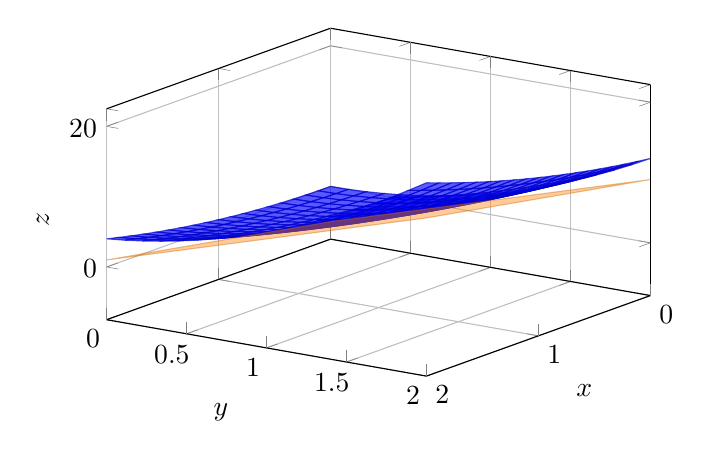
\begin{tikzpicture}\begin{axis}[domain=0:2,y domain=0:2]\addplot3[surf,opacity=.65,samples=19,colormap={blue}{color=(blue) color=(blue)}]{x^2+x*y+3*y^2};\addplot3[surf,opacity=.4,samples=2,colormap={orange}{color=(orange) color=(orange)}]{3*x+7*y-5};\end{axis}\end{tikzpicture}\end{center}
\begin{center}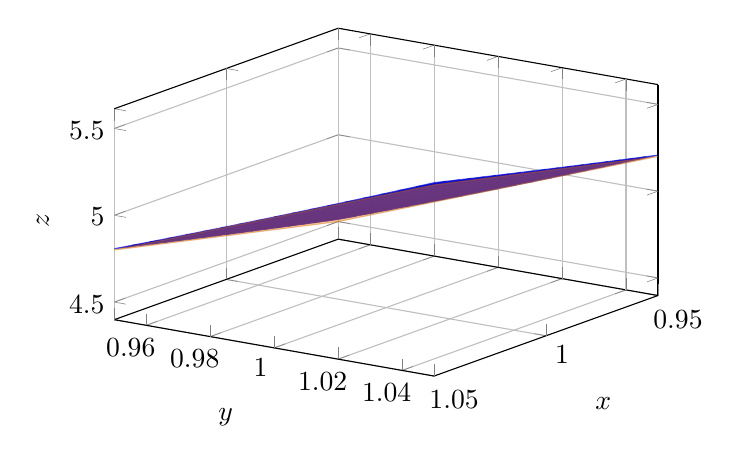
\begin{tikzpicture}\begin{axis}[domain=.95:1.05,y domain=.95:1.05]\addplot3[surf,opacity=.65,samples=19,colormap={blue}{color=(blue) color=(blue)}]{x^2+x*y+3*y^2};\addplot3[surf,opacity=.4,samples=2,colormap={orange}{color=(orange) color=(orange)}]{3*x+7*y-5};\end{axis}\end{tikzpicture}\end{center}
\ex{15}
\textbf{Question.} Explain differentiability of $f(x,y)=x^3y^2$ at $(-2,1)$ and find its linearization there.

\textbf{Worked solution.}
$f=x^3y^2$ is a polynomial, so its partials are continuous everywhere and it is differentiable at $(-2,1)$. There $f=-8$, $f_x=3x^2y^2=12$, and $f_y=2x^3y=-16$. Thus
\[\ans{L(x,y)=-8+12(x+2)-16(y-1)=12x-16y+32}.\]
\ex{25}
\textbf{Question.} Given $f(2,5)=6$, $f_x(2,5)=1$, and $f_y(2,5)=-1$, estimate $f(2.2,4.9)$ by linear approximation.

\textbf{Worked solution.}
At $(2,5)$, $f=6$, $f_x=1$, and $f_y=-1$. The increments are $dx=2.2-2=.2$ and $dy=4.9-5=-.1$. Hence
\[f(2.2,4.9)\approx6+1(.2)+(-1)(-.1)=\ans{6.3}.\]
This is a linear estimate; differentiability does not specify the exact remainder without more information about $f$.
\ex{31}
\textbf{Question.} Find the differential of $m=p^5q^3$.

\textbf{Worked solution.}
For $m=p^5q^3$, $m_p=5p^4q^3$ and $m_q=3p^5q^2$. Therefore
\[\ans{dm=5p^4q^3\,dp+3p^5q^2\,dq}.\]
\clearpage\section*{14.5 The Chain Rule}\addcontentsline{toc}{section}{14.5 The Chain Rule}
\ex{1}
\textbf{Question.} Find $dz/dt$ by both the chain rule and direct substitution for $z=x^2y+xy^2$, $x=3t$, $y=t^2$.

\textbf{Worked solution.}
\textbf{Chain rule:} $z=x^2y+xy^2$ gives $z_x=2xy+y^2$, $z_y=x^2+2xy$. With $x=3t$, $y=t^2$, $x'=3$, $y'=2t$,
\[\frac{dz}{dt}=(6t^3+t^4)3+(9t^2+6t^3)2t=\ans{36t^3+15t^4}.\]
\textbf{Substitution:} $z=(3t)^2t^2+(3t)(t^2)^2=9t^4+3t^5$, so $z'=36t^3+15t^4$, agreeing exactly.
\ex{3}
\textbf{Question.} Use the chain rule for $z=xy^3-x^3y$, $x=t^2+1$, $y=t^2-1$.

\textbf{Worked solution.}
For $z=xy^3-x^3y$, $z_x=y^3-3x^2y$, $z_y=3xy^2-x^3$. Since $x=t^2+1$, $y=t^2-1$, both derivatives are $2t$. Thus
\[\ans{z'=2t[y^3-3x^2y+3xy^2-x^3]},\quad x=t^2+1,\ y=t^2-1.\]
For a simplified form, $xy=t^4-1$ and $y^2-x^2=-4t^2$, so $z=xy(y^2-x^2)=-4t^6+4t^2$ and $\ans{z'=-24t^5+8t}$.
\ex{5}
\textbf{Question.} Use the chain rule for $z=\sin x\cos y$, $x=\sqrt t$, $y=1/t$.

\textbf{Worked solution.}
For $z=\sin x\cos y$, $z_x=\cos x\cos y$, $z_y=-\sin x\sin y$. With $x=\sqrt t$ and $y=1/t$, $x'=1/(2\sqrt t)$ and $y'=-1/t^2$, so for $t>0$,
\[\ans{z'=\frac{\cos\sqrt t\cos(1/t)}{2\sqrt t}+\frac{\sin\sqrt t\sin(1/t)}{t^2}}.\]
\ex{7}
\textbf{Question.} Use the chain rule for $w=xe^{y/z}$, $x=t^2$, $y=1-t$, $z=1+2t$.

\textbf{Worked solution.}
For $w=xe^{y/z}$, the partials are $w_x=e^{y/z}$, $w_y=(x/z)e^{y/z}$, and $w_z=-(xy/z^2)e^{y/z}$. The inner functions give $x'=2t$, $y'=-1$, $z'=2$. Therefore
\[w'=e^{y/z}\left(2t-\frac{x}{z}-\frac{2xy}{z^2}\right)
=\ans{e^{(1-t)/(1+2t)}\left(2t-\frac{3t^2}{(1+2t)^2}\right)},\quad t\ne-\tfrac12.\]
The simplification uses $z+2y=(1+2t)+2(1-t)=3$.
\ex{9}
\textbf{Question.} Find $z_s,z_t$ by both methods for $z=x^2+y^2$, $x=2s+3t$, $y=s+t$.

\textbf{Worked solution.}
\textbf{Chain rule:} for $z=x^2+y^2$, $z_s=2xx_s+2yy_s$ and $z_t=2xx_t+2yy_t$. With $x=2s+3t$, $y=s+t$,
\[z_s=4(2s+3t)+2(s+t)=\ans{10s+14t},\]
\[z_t=6(2s+3t)+2(s+t)=\ans{14s+20t}.\]
\textbf{Substitution:} $z=(2s+3t)^2+(s+t)^2=5s^2+14st+10t^2$. Its direct partials give the same answers.
\ex{11}
\textbf{Question.} Find $z_s,z_t$ for $z=(x-y)^5$, $x=s^2t$, $y=st^2$.

\textbf{Worked solution.}
$z=(x-y)^5$ has $z_x=5(x-y)^4$, $z_y=-5(x-y)^4$. For $x=s^2t$, $y=st^2$, the inner partials are $x_s=2st$, $y_s=t^2$, $x_t=s^2$, $y_t=2st$. Hence
\[\ans{z_s=5(s^2t-st^2)^4(2st-t^2)},\qquad
\ans{z_t=5(s^2t-st^2)^4(s^2-2st)}.\]
\ex{13}
\textbf{Question.} Find $z_s,z_t$ for $z=\ln(3x+2y)$, $x=s\sin t$, $y=t\cos s$.

\textbf{Worked solution.}
For $z=\ln(3x+2y)$, $z_x=3/(3x+2y)$ and $z_y=2/(3x+2y)$. With $x=s\sin t$, $y=t\cos s$,
\[x_s=\sin t,\ y_s=-t\sin s,\ x_t=s\cos t,\ y_t=\cos s.\]
Consequently, on $3s\sin t+2t\cos s>0$,
\[\ans{z_s=\frac{3\sin t-2t\sin s}{3s\sin t+2t\cos s}},\quad
\ans{z_t=\frac{3s\cos t+2\cos s}{3s\sin t+2t\cos s}}.\]
\ex{15}
\textbf{Question.} Find $z_s,z_t$ for $z=(\sin\theta)/r$, $r=st$, $\theta=s^2+t^2$.

\textbf{Worked solution.}
For $z=\sin\theta/r$, $z_r=-\sin\theta/r^2$ and $z_\theta=\cos\theta/r$. Since $r=st$, $\theta=s^2+t^2$, $r_s=t$, $r_t=s$, $\theta_s=2s$, and $\theta_t=2t$,
\[\ans{z_s=-\frac{\sin(s^2+t^2)}{s^2t}+\frac{2\cos(s^2+t^2)}t},\]
\[\ans{z_t=-\frac{\sin(s^2+t^2)}{st^2}+\frac{2\cos(s^2+t^2)}s},\qquad st\ne0.\]
\ex{17}
\textbf{Question.} Find $p\prime(2)$ for $p(t)=f(g(t),h(t))$ using $g(2)=4$, $g\prime(2)=-3$, $h(2)=5$, $h\prime(2)=6$, $f_x(4,5)=2$, and $f_y(4,5)=8$.

\textbf{Worked solution.}
The chain rule for $p(t)=f(g(t),h(t))$ gives $p'=f_x(g,h)g'+f_y(g,h)h'$. At $t=2$, $(g,h)=(4,5)$, so
\[p'(2)=f_x(4,5)g'(2)+f_y(4,5)h'(2)=2(-3)+8(6)=\ans{42}.\]
\ex{19}
\textbf{Question.} For $g(u,v)=f(e^u+\sin v,e^u+\cos v)$, use the supplied table to find $g_u(0,0)$ and $g_v(0,0)$. The relevant row has $f_x(1,2)=2$, $f_y(1,2)=5$.

\textbf{Worked solution.}
For $g(u,v)=f(e^u+\sin v,e^u+\cos v)$, $(u,v)=(0,0)$ maps to $(x,y)=(1,2)$. The relevant table entries are $f_x(1,2)=2$, $f_y(1,2)=5$, not the entries at $(0,0)$. Now
\[g_u=f_xe^u+f_ye^u\Rightarrow\ans{g_u(0,0)=2+5=7},\]
\[g_v=f_x\cos v-f_y\sin v\Rightarrow\ans{g_v(0,0)=2(1)-5(0)=2}.\]
\ex{21}
\textbf{Question.} Draw the dependency tree and write the chain rule for $u=f(x,y)$, with $x=x(r,s,t)$ and $y=y(r,s,t)$.

\textbf{Worked solution.}
The dependency tree has root $u$, children $x,y$, and each child has leaves $r,s,t$. Sum the derivative products along all paths to each leaf:
\[\ans{u_r=f_x\,x_r+f_y\,y_r},\quad\ans{u_s=f_x\,x_s+f_y\,y_s},\quad\ans{u_t=f_x\,x_t+f_y\,y_t}.\]
Each term is a product of derivatives along one path through the dependency tree. The tree can be drawn as
\begin{center}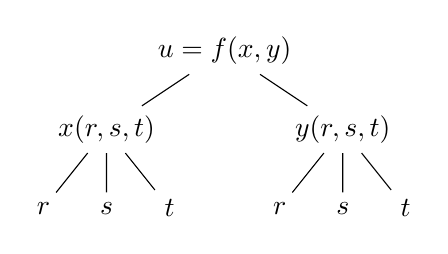
\begin{tikzpicture}[level distance=1cm,sibling distance=3cm]\node{$u=f(x,y)$} child{node{$x(r,s,t)$} child[sibling distance=.8cm]{node{$r$}} child[sibling distance=.8cm]{node{$s$}} child[sibling distance=.8cm]{node{$t$}}} child{node{$y(r,s,t)$} child[sibling distance=.8cm]{node{$r$}} child[sibling distance=.8cm]{node{$s$}} child[sibling distance=.8cm]{node{$t$}}};\end{tikzpicture}\end{center}
\ex{23}
\textbf{Question.} Draw the dependency tree and write the chain rule for $T=F(p,q,r)$, where each of $p,q,r$ depends on $x,y,z$.

\textbf{Worked solution.}
The tree is $T\to(p,q,r)$, with each of $p,q,r\to(x,y,z)$. There are three paths to each independent variable, yielding
\[\ans{T_x=F_p\,p_x+F_q\,q_x+F_r\,r_x},\]
\[\ans{T_y=F_p\,p_y+F_q\,q_y+F_r\,r_y},\quad
\ans{T_z=F_p\,p_z+F_q\,q_z+F_r\,r_z}.\]
\begin{center}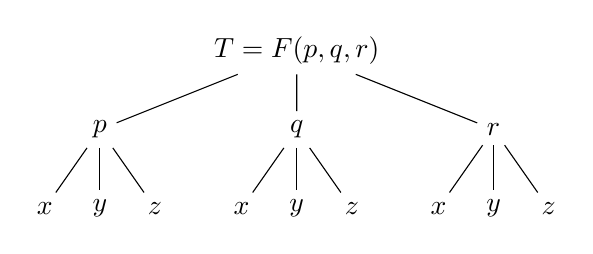
\begin{tikzpicture}[level distance=1cm,sibling distance=2.5cm]\node{$T=F(p,q,r)$} child{node{$p$} child[sibling distance=.7cm]{node{$x$}} child[sibling distance=.7cm]{node{$y$}} child[sibling distance=.7cm]{node{$z$}}} child{node{$q$} child[sibling distance=.7cm]{node{$x$}} child[sibling distance=.7cm]{node{$y$}} child[sibling distance=.7cm]{node{$z$}}} child{node{$r$} child[sibling distance=.7cm]{node{$x$}} child[sibling distance=.7cm]{node{$y$}} child[sibling distance=.7cm]{node{$z$}}};\end{tikzpicture}\end{center}
\ex{25}
\textbf{Question.} Find $z_s,z_t,z_u$ at $(4,2,1)$ for $z=x^4+x^2y$, $x=s+2t-u$, $y=stu^2$.

\textbf{Worked solution.}
$z=x^4+x^2y$ gives $z_x=4x^3+2xy$, $z_y=x^2$. At $(s,t,u)=(4,2,1)$, $x=s+2t-u=7$ and $y=stu^2=8$, so $z_x=4(343)+2(7)(8)=1484$, $z_y=49$. The inner partials are
\[x_s=1,\ x_t=2,\ x_u=-1,\quad y_s=tu^2=2,\ y_t=su^2=4,\ y_u=2stu=16.\]
Thus $\ans{z_s=1484+49(2)=1582}$, $\ans{z_t=1484(2)+49(4)=3164}$, and $\ans{z_u=-1484+49(16)=-700}$.
\ex{27}
\textbf{Question.} Find $w_r,w_\theta$ at $r=2$, $\theta=\pi/2$ for $w=xy+yz+zx$, $x=r\cos\theta$, $y=r\sin\theta$, $z=r\theta$.

\textbf{Worked solution.}
For $w=xy+yz+zx$, $w_x=y+z$, $w_y=x+z$, $w_z=x+y$. At $r=2$, $\theta=\pi/2$, $(x,y,z)=(0,2,\pi)$, so these partials are $2+\pi,\pi,2$. Also
\[x_r=\cos\theta=0,\ y_r=\sin\theta=1,\ z_r=\theta=\pi/2,\]
\[x_\theta=-r\sin\theta=-2,\ y_\theta=r\cos\theta=0,\ z_\theta=r=2.\]
Therefore $\ans{w_r=(2+\pi)0+\pi+2(\pi/2)=2\pi}$ and $\ans{w_\theta=(2+\pi)(-2)+\pi0+2(2)=-2\pi}$.
\ex{29}
\textbf{Question.} Find $N_u,N_v,N_w$ at $(2,3,4)$ for $N=(p+q)/(p+r)$, $p=u+vw$, $q=v+uw$, $r=w+uv$.

\textbf{Worked solution.}
$N=(p+q)/(p+r)$ has partials
\[N_p=\frac{r-q}{(p+r)^2},\quad N_q=\frac1{p+r},\quad N_r=-\frac{p+q}{(p+r)^2}.\]
At $(u,v,w)=(2,3,4)$, $(p,q,r)=(u+vw,v+uw,w+uv)=(14,11,10)$. Thus $(N_p,N_q,N_r)=(-1/576,1/24,-25/576)$. The inner derivative vectors are
\[(p_u,q_u,r_u)=(1,4,3),\quad(p_v,q_v,r_v)=(4,1,2),\quad(p_w,q_w,r_w)=(3,2,1).\]
Take their dot products with the outer partials:
\[\ans{N_u=\frac{-1+96-75}{576}=\frac5{144}},\quad
\ans{N_v=\frac{-4+24-50}{576}=-\frac5{96}},\quad
\ans{N_w=\frac{-3+48-25}{576}=\frac5{144}}.\]
\ex{31}
\textbf{Question.} Find $dy/dx$ implicitly from $y\cos x=x^2+y^2$.

\textbf{Worked solution.}
For $F(x,y)=y\cos x-x^2-y^2=0$, $F_x=-y\sin x-2x$ and $F_y=\cos x-2y$. The implicit derivative is
\[\ans{\frac{dy}{dx}=-\frac{F_x}{F_y}=\frac{y\sin x+2x}{\cos x-2y}},\qquad F_y\ne0.\]
\ex{33}
\textbf{Question.} Find $dy/dx$ implicitly from $\arctan(x^2y)=x+xy^2$.

\textbf{Worked solution.}
Let $F=\arctan(x^2y)-x-xy^2=0$, and $D=1+x^4y^2$. Then
\[F_x=\frac{2xy}{D}-1-y^2,\qquad F_y=\frac{x^2}{D}-2xy.\]
Apply $y'=-F_x/F_y$ and multiply numerator and denominator by $D$:
\[\ans{y'=\frac{(1+y^2)(1+x^4y^2)-2xy}{x^2-2xy(1+x^4y^2)}},\qquad F_y\ne0.\]
\clearpage\section*{14.6 Directional Derivatives and the Gradient Vector}\addcontentsline{toc}{section}{14.6 Directional Derivatives and the Gradient Vector}
\noindent For a unit direction $u$, $D_uf=\nabla f\cdot u$. A supplied direction vector $v$ must first be normalized to $u=v/|v|$; otherwise the result includes an unintended speed factor.
\ex{5}
\textbf{Question.} Find the directional derivative of $f(x,y)=y\cos(xy)$ at $(0,1)$ in the direction $\theta=\pi/4$.

\textbf{Worked solution.}
$f=y\cos(xy)$ gives $f_x=-y^2\sin(xy)$ and $f_y=\cos(xy)-xy\sin(xy)$. At $(0,1)$, $\nabla f=\vv{0,1}$. With $\theta=\pi/4$, $u=\vv{1/\sqrt2,1/\sqrt2}$, so $\ans{D_uf=1/\sqrt2}$.
\ex{7}
\textbf{Question.} Find the directional derivative of $f(x,y)=\arctan(xy)$ at $(2,-3)$ in the direction $\theta=3\pi/4$.

\textbf{Worked solution.}
For $f=\arctan(xy)$,
\[\nabla f=\frac{\vv{y,x}}{1+x^2y^2},\qquad\nabla f(2,-3)=\vv{-3/37,2/37}.\]
With $u=\vv{\cos(3\pi/4),\sin(3\pi/4)}=\vv{-1/\sqrt2,1/\sqrt2}$, the dot product is $\ans{5/(37\sqrt2)}$.
\ex{9}
\textbf{Question.} Find $\nabla f$, its value at $P$, and $D_uf(P)$ for $f=x/y$, $P=(2,1)$, $u=\vv{3/5,4/5}$.

\textbf{Worked solution.}
\begin{enumerate}[label=(\alph*)]
\item $f=x/y$ gives $\ans{\nabla f=\vv{1/y,-x/y^2}}$, $y\ne0$.
\item At $P=(2,1)$, $\ans{\nabla f(P)=\vv{1,-2}}$.
\item The given $u=\vv{3/5,4/5}$ is unit because $(3/5)^2+(4/5)^2=1$. Thus $D_uf(P)=1(3/5)-2(4/5)=\ans{-1}$.
\end{enumerate}
\ex{11}
\textbf{Question.} Find $\nabla f$, its value at $P$, and $D_uf(P)$ for $f=x^2yz-xyz^3$, $P=(2,-1,1)$, $u=\vv{0,4/5,-3/5}$.

\textbf{Worked solution.}
\begin{enumerate}[label=(\alph*)]
\item For $f=x^2yz-xyz^3$,
\[\ans{\nabla f=\vv{2xyz-yz^3,x^2z-xz^3,x^2y-3xyz^2}}.\]
\item Substitution of $(2,-1,1)$ gives $\ans{\nabla f(P)=\vv{-3,2,2}}$.
\item With the unit $u=\vv{0,4/5,-3/5}$, $D_uf(P)=-3(0)+2(4/5)+2(-3/5)=\ans{2/5}$.
\end{enumerate}
\ex{15}
\textbf{Question.} Find the directional derivative of $g(s,t)=s\sqrt t$ at $(2,4)$ in the direction $v=\vv{2,-1}$.

\textbf{Worked solution.}
$g(s,t)=s\sqrt t$ gives $\nabla g=\vv{\sqrt t,s/(2\sqrt t)}$, hence $\nabla g(2,4)=\vv{2,1/2}$. Normalize $v=\vv{2,-1}$ to $u=\vv{2,-1}/\sqrt5$. Therefore
\[\ans{D_ug(2,4)=\frac{2(2)+(1/2)(-1)}{\sqrt5}=\frac7{2\sqrt5}}.\]
\ex{21}
\textbf{Question.} For $f=x^2y^2-y^3$, find the directional derivative at $P=(1,2)$ toward $Q=(-3,5)$.

\textbf{Worked solution.}
The direction from $P=(1,2)$ to $Q=(-3,5)$ is $Q-P=\vv{-4,3}$, of length $5$. For $f=x^2y^2-y^3$, $\nabla f=\vv{2xy^2,2x^2y-3y^2}$, so $\nabla f(P)=\vv{8,-8}$. Thus
\[\ans{D_uf(P)=\vv{8,-8}\cdot\frac{\vv{-4,3}}5=\frac{-32-24}5=-\frac{56}5}.\]
\ex{29}
\textbf{Question.} Find the maximum rate of change of $f=\sin(xy)$ at $(1,0)$ and its direction.

\textbf{Worked solution.}
$f=\sin(xy)$ gives $\nabla f=\vv{y\cos(xy),x\cos(xy)}$ and $\nabla f(1,0)=\vv{0,1}$. By Cauchy--Schwarz, $\nabla f\cdot u\le|\nabla f|$ for unit $u$, with equality in its direction. Hence the maximum rate is $\ans{1}$, occurring in direction $\ans{\vv{0,1}}$.
\ex{41}
\textbf{Question.} Given $A=(1,3)$, $B=(3,3)$, $C=(1,7)$, $D=(6,15)$ and directional derivatives $3$ toward $B$ and $26$ toward $C$, find the derivative at $A$ toward $D$.

\textbf{Worked solution.}
$\overrightarrow{AB}=\vv{2,0}$ and $\overrightarrow{AC}=\vv{0,4}$. Their unit directions are $\vv{1,0}$ and $\vv{0,1}$, so the supplied directional derivatives imply $f_x(A)=3$ and $f_y(A)=26$. Now $\overrightarrow{AD}=\vv{5,12}$ has length $13$. Therefore
\[\ans{D_{AD}f(A)=\vv{3,26}\cdot\frac{\vv{5,12}}{13}=\frac{15+312}{13}=\frac{327}{13}}.\]
\ex{43}
\textbf{Question.} Prove the gradient rules for $au+bv$, $uv$, $u/v$, and $u^n$, with $a,b$ constant.

\textbf{Worked solution.}
Each gradient identity follows component by component from the corresponding one-variable derivative rule:
\begin{enumerate}[label=(\alph*)]
\item $(au+bv)_x=au_x+bv_x$ and $(au+bv)_y=au_y+bv_y$, so $\ans{\nabla(au+bv)=a\nabla u+b\nabla v}$.
\item $(uv)_x=u_xv+uv_x$, $(uv)_y=u_yv+uv_y$. Collecting the two components gives $\ans{\nabla(uv)=v\nabla u+u\nabla v}$.
\item For $v\ne0$, $(u/v)_x=(vu_x-uv_x)/v^2$ and $(u/v)_y=(vu_y-uv_y)/v^2$, hence
\[\ans{\nabla(u/v)=(v\nabla u-u\nabla v)/v^2}.\]
\item $(u^n)_x=nu^{n-1}u_x$, $(u^n)_y=nu^{n-1}u_y$, giving $\ans{\nabla(u^n)=nu^{n-1}\nabla u}$ wherever that power is differentiable.
\end{enumerate}
\ex{45}
\textbf{Question.} Calculate $D_u^2f(2,1)$ for $f=x^3+5x^2y+y^3$ and $u=\vv{3/5,4/5}$.

\textbf{Worked solution.}
For $f=x^3+5x^2y+y^3$ and $u=\vv{3/5,4/5}$,
\[D_uf=\frac35(3x^2+10xy)+\frac45(5x^2+3y^2)
=\frac{29}5x^2+6xy+\frac{12}5y^2.\]
Apply the same directional derivative again:
\[D_u^2f=\frac35\left(\frac{58}5x+6y\right)+\frac45\left(6x+\frac{24}5y\right)
=\frac{294}{25}x+\frac{186}{25}y.\]
At $(2,1)$ this gives $\ans{D_u^2f(2,1)=774/25}$.
\ex{51}
\textbf{Question.} Find the tangent plane and normal line to $x+y+z=e^{xyz}$ at $(0,0,1)$.

\textbf{Worked solution.}
Put $F=x+y+z-e^{xyz}$, so the surface is $F=0$. Its gradient is
\[\nabla F=\vv{1-yze^{xyz},1-xze^{xyz},1-xye^{xyz}}.\]
At $P=(0,0,1)$, $\nabla F(P)=\vv{1,1,1}\ne0$.
\begin{enumerate}[label=(\alph*)]
\item The plane is $\nabla F(P)\cdot\vv{x,y,z-1}=0$, or $\ans{x+y+z=1}$.
\item The normal line is $\ans{\vv{x,y,z}=\vv{0,0,1}+t\vv{1,1,1}}$.
\end{enumerate}
\ex{57}
\textbf{Question.} Derive the tangent-plane equation to $x^2/a^2+y^2/b^2+z^2/c^2=1$ at $(x_0,y_0,z_0)$.

\textbf{Worked solution.}
Use $F=x^2/a^2+y^2/b^2+z^2/c^2$. Its gradient at $P$ is $\vv{2x_0/a^2,2y_0/b^2,2z_0/c^2}$. Therefore the tangent plane is
\[\frac{x_0(x-x_0)}{a^2}+\frac{y_0(y-y_0)}{b^2}+\frac{z_0(z-z_0)}{c^2}=0.\]
Move the constant terms to the right. Because $P$ is on the ellipsoid, their sum is $1$, yielding
\[\ans{\frac{xx_0}{a^2}+\frac{yy_0}{b^2}+\frac{zz_0}{c^2}=1}.\]
\ex{61}
\textbf{Question.} Find any points on $x^2-y^2-z^2=1$ whose tangent plane is parallel to $z=x+y$.

\textbf{Worked solution.}
The plane $z=x+y$ has normal $\vv{1,1,-1}$. On $x^2-y^2-z^2=1$, the normal is $\vv{2x,-2y,-2z}$. Parallel normals would require $\vv{2x,-2y,-2z}=\lambda\vv{1,1,-1}$, hence $(x,y,z)=(\lambda/2,-\lambda/2,\lambda/2)$. Substitution into the surface gives $-\lambda^2/4=1$, impossible over the reals. Therefore $\ans{\text{there are no such points}}$.
\clearpage\section*{14.7 Maximum and Minimum Values}\addcontentsline{toc}{section}{14.7 Maximum and Minimum Values}
\noindent At a critical point, use $D=f_{xx}f_{yy}-f_{xy}^2$. If $D>0$, the sign of $f_{xx}$ distinguishes a minimum (positive) from a maximum (negative); $D<0$ means a saddle.
\ex{5}
\textbf{Question.} Find and classify the critical points of $f=x^2+xy+y^2+y$.

\textbf{Worked solution.}
For $f=x^2+xy+y^2+y$, $f_x=2x+y=0$ and $f_y=x+2y+1=0$. The first equation gives $y=-2x$; the second becomes $-3x+1=0$. Thus $(x,y)=(1/3,-2/3)$. Since $f_{xx}=2$, $f_{yy}=2$, $f_{xy}=1$, $D=3>0$: a minimum. Its value is $1/9-2/9+4/9-2/3=\ans{-1/3}$. In fact, with $h=x-1/3$, $k=y+2/3$, $f+1/3=h^2+hk+k^2\ge0$, so the minimum is absolute. There are no maxima or saddles.
\ex{9}
\textbf{Question.} Find and classify the critical points of $f=(x-y)(1-xy)$.

\textbf{Worked solution.}
Expand $f=(x-y)(1-xy)=x-y-x^2y+xy^2$. Then
\[f_x=1-2xy+y^2=0,\quad f_y=-1-x^2+2xy=0.\]
Adding gives $y^2-x^2=0$. If $y=x$, the equations give $1-x^2=0$, so $(1,1)$ and $(-1,-1)$. If $y=-x$, $f_x=1+3x^2$ cannot vanish. The Hessian entries are $-2y,2x,-2x+2y$. At both points $D=(-2y)(2x)-0=-4<0$, so both are saddles, with value $0$. No local extrema exist.
\ex{15}
\textbf{Question.} Find and classify the critical points of $f=x^4-2x^2+y^3-3y$.

\textbf{Worked solution.}
$f=x^4-2x^2+y^3-3y$ gives $f_x=4x(x^2-1)=0$ and $f_y=3(y^2-1)=0$. Thus $x=0,\pm1$ and $y=\pm1$, making six critical points. The Hessian is diagonal, with entries $12x^2-4$ and $6y$.
\begin{center}\begin{tabular}{lll}\toprule Point&Signs of diagonal entries&Classification and value\\\midrule
$(0,-1)$&$-,-$&local maximum $2$\\
$(1,1),(-1,1)$&$+,+$&local minima $-3$\\
$(0,1)$&$-,+$&saddle $-2$\\
$(1,-1),(-1,-1)$&$+,-$&saddles $1$\\\bottomrule\end{tabular}\end{center}
Because $y^3-3y$ is unbounded in both signs, no absolute extrema exist on the whole plane.
\ex{31}
\textbf{Question.} Find the critical points to three decimal places and classify them for $f=x^4+y^3-3x^2+y^2+x-2y+1$; determine whether the full graph has highest or lowest points.

\textbf{Worked solution.}
$f=x^4+y^3-3x^2+y^2+x-2y+1$ has
\[f_x=4x^3-6x+1=0,\quad f_y=3y^2+2y-2=0.\]
The second equation has exact roots $y=(-1\pm\sqrt7)/3$. Solving the cubic numerically gives $x\approx-1.300840,.169938,1.130901$. There are six combinations. Since $f_{xy}=0$, inspect $f_{xx}=12x^2-6$ and $f_{yy}=6y+2$.
\begin{center}\begin{tabular}{rrrl}\toprule $x$&$y$&$f(x,y)$&Type\\\midrule
$-1.301$&$-1.215$&$-0.401$&saddle\\
$-1.301$&$.549$&$-3.145$&local minimum\\
$.170$&$-1.215$&$3.197$&local maximum\\
$.170$&$.549$&$.453$&saddle\\
$1.131$&$-1.215$&$2.042$&saddle\\
$1.131$&$.549$&$-.701$&local minimum\\
\bottomrule\end{tabular}\end{center}
The function tends to $+\infty$ as $y\to+\infty$ and to $-\infty$ as $y\to-\infty$ with $x$ fixed, so it has no highest or lowest point on its full graph. The table's extrema are local.
\ex{33}
\textbf{Question.} Find absolute extrema of $f=x^2+y^2-2x$ on the closed triangle with vertices $(2,0)$, $(0,2)$, $(0,-2)$.

\textbf{Worked solution.}
$f=x^2+y^2-2x=(x-1)^2+y^2-1$. The critical point $(1,0)$ lies in the triangle and gives the absolute minimum $\ans{-1}$.
Check all three edges for the maximum. On $x=0$, $-2\le y\le2$, $f=y^2$, ranging from $0$ to $4$. On the upper sloping edge $y=2-x$, $0\le x\le2$,
\[f=x^2+(2-x)^2-2x=2x^2-6x+4.\]
Its derivative is $4x-6$, giving $x=3/2$ and value $-1/2$; endpoint values are $4,0$. The lower edge $y=x-2$ gives the same polynomial and values. Comparing all candidates gives maximum $\ans{4}$ at $(0,\pm2)$, and minimum $-1$ at $(1,0)$.
\ex{35}
\textbf{Question.} Find absolute extrema of $f=x^2+y^2+x^2y+4$ on $|x|\le1$, $|y|\le1$.

\textbf{Worked solution.}
On $|x|,|y|\le1$, $f=x^2+y^2+x^2y+4$. The equations are $f_x=2x(1+y)=0$ and $f_y=2y+x^2=0$. In the interior, $1+y>0$, so the sole critical point is $(0,0)$ with $f=4$. Also $f=4+y^2+x^2(1+y)\ge4$ everywhere in the square, proving its absolute minimality.
On $x=\pm1$, $f=y^2+y+5$, whose critical value at $y=-1/2$ is $19/4$ and endpoint values are $5,7$. On $y=1$, $f=5+2x^2$, from $5$ to $7$; on $y=-1$, $f=5$ identically. Thus $\ans{\min f=4\text{ at }(0,0),\quad\max f=7\text{ at }(\pm1,1)}$.
\ex{37}
\textbf{Question.} Find absolute extrema of $f=x^2+2y^2-2x-4y+1$ on $0\le x\le2$, $0\le y\le3$.

\textbf{Worked solution.}
Complete the squares:
\[f=x^2+2y^2-2x-4y+1=(x-1)^2+2(y-1)^2-2.\]
On $0\le x\le2$, $0\le y\le3$, the minimum is $\ans{-2}$ at $(1,1)$. To maximize, $(x-1)^2\le1$ and $(y-1)^2\le4$, so $f\le1+8-2=7$. Both bounds are attained at $(0,3)$ and $(2,3)$; hence $\ans{\max f=7}$ there.
\ex{41}
\textbf{Question.} Show that $f=-(x^2-1)^2-(x^2y-x-1)^2$ has just two critical points, both local maxima, and no local minimum; graph it to explain this behavior.

\textbf{Worked solution.}
Let $A=x^2-1$, $B=x^2y-x-1$, so $f=-A^2-B^2$. Then
\[f_y=-2Bx^2,\qquad f_x=-4xA-2B(2xy-1).\]
If $x=0$, $B=-1$ and $f_x=-2\ne0$, so there is no critical point there. Otherwise $f_y=0$ forces $B=0$, and then $f_x=0$ forces $A=0$. Thus $x=1,y=2$ or $x=-1,y=0$. At both points $f=0$, while $f\le0$ everywhere, so both are absolute (and local) maxima.
To prove there are no local minima, any local minimum of this smooth function would be critical; the only two critical points are strict maxima. Their strictness follows because $A=B=0$ occurs only at those isolated points. A graph of the narrow ridge $B=0$, namely $y=(x+1)/x^2$, explains how the two peaks can be separated without another critical point: the ridge escapes to infinity as $x\to0$.
\surf{domain=-2:-.25,y domain=-1:3,zmin=-15,zmax=0}{x}{y}{-(x^2-1)^2-(x^2*y-x-1)^2}
\surf{domain=.25:2,y domain=-1:4,zmin=-15,zmax=0}{x}{y}{-(x^2-1)^2-(x^2*y-x-1)^2}

The following two closer views retain both peaks without clipping the narrow ridge.
\surf{domain=-1.25:-.75,y domain=-.75:.75,zmin=-2,zmax=.1}{x}{y}{-(x^2-1)^2-(x^2*y-x-1)^2}
\surf{domain=.75:1.25,y domain=1.25:2.75,zmin=-2,zmax=.1}{x}{y}{-(x^2-1)^2-(x^2*y-x-1)^2}
\ex{43}
\textbf{Question.} Find the shortest distance from $(2,0,-3)$ to the plane $x+y+z=1$.

\textbf{Worked solution.}
On $x+y+z=1$, minimize squared distance from $(2,0,-3)$:
\[d^2=(x-2)^2+y^2+(1-x-y+3)^2=(x-2)^2+y^2+(4-x-y)^2.\]
Its equations are $2(x-2)-2(4-x-y)=0$ and $2y-2(4-x-y)=0$, giving $2x+y=6$, $x+2y=4$. Thus $x=8/3$, $y=2/3$, $z=-7/3$. The displacement is $\vv{2/3,2/3,2/3}$, so $\ans{d=2/\sqrt3}$. The squared-distance quadratic is strictly convex, ensuring a minimum.
\ex{45}
\textbf{Question.} Find the points on $z^2=x^2+y^2$ closest to $(4,2,0)$.

\textbf{Worked solution.}
On the cone, $z^2=x^2+y^2$. Therefore squared distance from $(4,2,0)$ is
\[d^2=(x-4)^2+(y-2)^2+z^2
=2x^2+2y^2-8x-4y+20
=2(x-2)^2+2(y-1)^2+10.\]
It is minimized at $x=2$, $y=1$, and the cone condition gives $z=\pm\sqrt5$. The closest points are $\ans{(2,1,\sqrt5),(2,1,-\sqrt5)}$, both at distance $\sqrt{10}$.
\ex{47}
\textbf{Question.} Find three positive numbers with sum $100$ and maximum product.

\textbf{Worked solution.}
Let positive numbers be $x,y,z$ with $x+y+z=100$. Substitute $z=100-x-y$ into $P=xyz$:
\[P_x=y(100-2x-y)=0,\quad P_y=x(100-x-2y)=0.\]
Since $x,y>0$, $2x+y=100$ and $x+2y=100$, hence $x=y=z=100/3$. The Hessian there has $P_{xx}=P_{yy}=-200/3$ and $P_{xy}=-100/3$, so $D=10000/3>0$: a local maximum. On the closed triangle $x,y\ge0$, $x+y\le100$, $P=0$ on the boundary, while its only interior critical value is positive. Thus it is the absolute maximum $\ans{(100/3)^3=1000000/27}$.
\clearpage\section*{14.8 Lagrange Multipliers}\addcontentsline{toc}{section}{14.8 Lagrange Multipliers}
\ex{3}
\textbf{Question.} Use Lagrange multipliers to find extrema of $f=x^2-y^2$ subject to $x^2+y^2=1$.

\textbf{Worked solution.}
For $f=x^2-y^2$ on $g=x^2+y^2=1$, the multiplier equations are
\[2x=2\lambda x,\qquad-2y=2\lambda y,\qquad x^2+y^2=1.\]
If both $x$ and $y$ were nonzero, the first would give $\lambda=1$ and the second $\lambda=-1$, impossible. Thus $x=0$ or $y=0$. With $x=0$, $y=\pm1$ and $f=-1$; with $y=0$, $x=\pm1$ and $f=1$. The circle is compact and the constraint gradient never vanishes on it, so these candidates contain both global extrema:
\[\ans{\max f=1\text{ at }(\pm1,0),\qquad\min f=-1\text{ at }(0,\pm1)}.\]
\ex{7}
\textbf{Question.} Use Lagrange multipliers to find extrema of $f=2x^2+6y^2$ subject to $x^4+3y^4=1$.

\textbf{Worked solution.}
For $f=2x^2+6y^2$ on $g=x^4+3y^4=1$, the equations are
\[4x=4\lambda x^3,\quad12y=12\lambda y^3,\quad x^4+3y^4=1.\]
If $x=0$, then $y=\pm3^{-1/4}$ and $f=2\sqrt3$. If $y=0$, then $x=\pm1$ and $f=2$. If both are nonzero, dividing gives $1=\lambda x^2=\lambda y^2$, so $x^2=y^2$. The constraint becomes $4x^4=1$, hence $x^2=y^2=1/2$ and $f=1+3=4$. The level set is closed and bounded, and $\nabla g=\vv{4x^3,12y^3}$ cannot vanish on it. Comparing all cases yields
\[\ans{\min f=2\text{ at }(\pm1,0)},\qquad
\ans{\max f=4\text{ at }(\pm1/\sqrt2,\pm1/\sqrt2)},\]
with independent choices of the two signs.
\ex{23}
\textbf{Question.} For $f=x^2+y^2$ subject to $xy=1$, find the minimum by Lagrange multipliers and explain why there is no maximum.

\textbf{Worked solution.}
For $f=x^2+y^2$ with $xy=1$, the equations are $2x=\lambda y$ and $2y=\lambda x$. Neither coordinate is zero. Multiplying the first by $x$ and the second by $y$ gives $2x^2=\lambda xy=2y^2$. Thus $y=\pm x$, and $xy=1>0$ permits only $y=x$, yielding $(1,1)$ and $(-1,-1)$, both with $f=2$. Also
\[x^2+y^2=(x-y)^2+2xy=(x-y)^2+2\ge2,\]
so the absolute minimum is $\ans{2}$ at those points. There is no maximum: along the constraint $(x,y)=(t,1/t)$, $t>0$, $f=t^2+t^{-2}\to\infty$ as $t\to\infty$. This explicitly distinguishes existence of a minimum from existence of a maximum on an unbounded constraint.
\end{document}
